\chapter{Plataforma de desarrollo}
\label{cap:capitulo3}

En este capítulo se detalla sobre qué tecnologías se ha utilizado durante el desarrollo de este trabajo junto con el lenguaje de programación y las librerías utilizadas.
\section{Lenguaje de programación}
\label{sec:programación}
\subsection{Python}
\label{sec:python}
Para el desarrollo de este TFG, hemos utilizado como lenguaje de programación Python. Python\footnote{\url{https://www.python.org/}} es un lenguaje de programación interpretado, 
de tipado dinámico y orientado a objetos,
utilizado para el desarrollo de software, aplicaciones web, data science y machine learning (ML).  
Fue creado por Guido van Rossum\footnote{\url{https://gvnrossum.github.io/}} en 1989, el nombre de "Python" se inspiró en el programa de televisión británico 
"Monty Python's Flying Circus".

Este lenguaje con los tiempos se ha convertido en uno de los lenguajes más populares del mundo, esto se puede deber a su sintaxis sencilla, clara y legible, aparte 
de estos beneficios también presenta una amplia gama de bibliotecas y marcos de trabajo. Además,se trata de un lenguaje de programación 'open source' (código abierto) y está disponible bajo
una licencia de código abierto aprobada por la Iniciativa de Código Abierto (OSI), esto significa que Python es libre de usar, distribuir y modificar, incluso para uso
comercial.

En el caso de este TFG, se utiliza Python3 para todo el desarrollo del código junto con el middleware robótico ROS (véase la sección \ref{sec:ros}) y para el desarrollo
de los diferentes algoritmos. 

\begin{code}[h]
\begin{lstlisting}[language=Python]
  def factorial(n):
    if n == 0:
        return 1
    else:
        return n * factorial(n-1)
    print(factorial(5))  # Output: 120

\end{lstlisting}
\caption[Ejemplo de código en Python de una función para calcular el factorial de un número]{Ejemplo de código en Python de una función para calcular el factorial de un número}
\label{cod:codejemplo}
\end{code}  
Para el desarrollo del sistema de percepción, se ha  utilizado varías librerías mediante el lenguaje de programación Python para poder
percibir el entorno en el que se va a estar trabajando. 
\subsubsection{OpenCV}
\label{sec:OpenCV}
OpenCV (Open Source Computer Vision Library) es una biblioteca de open source dedicada para el tratamiento de imágenes y aprendizaje automático. Fue desarrollada por Intel y lanzada en 
el año 2000 y esta disponible para todos los públicos tanto para uso comercial como para uso personal\footnote{\url{https://opencv.org/}}.
Ofrece diferentes tareas como procesamiento de imágenes, detención de objetos, extracción de características, reconocimiento facial, estimación de movimiento entre otras. Además de ser
compatible para múltiples sistemas operativos como Windows, Linux, MacOS, Android e iOS, lo que hace que sea una librería muy versátil para el desarrollo de aplicaciones en diferentes
dispositivos y entornos. 

En este caso, se utiliza esta biblioteca para poder obtener la imagen mediante la cámara que va abordo del dron.

\begin{code}[h]
  \begin{lstlisting}[language=Python]
    import cv2

    imagen = cv2.imread('ruta/a/tu/imagen.jpg')
    cv2.imshow('Imagen', imagen)
    
    cv2.waitKey(0)
    cv2.destroyAllWindows()
    
  \end{lstlisting}
  \caption[Ejemplo de código en Python de operaciones básicas utilizando la librería OpenCv]{Ejemplo de código en Python de operaciones básicas utilizando la libreria OpenCv}
  \label{cod:Numpy}
  \end{code}  

\subsubsection{Numpy}
\label{sec:Numpy}

Numpy\footnote{\url{https://numpy.org/}} (Numerical Python) es una librería dedicada para el cálculo científico en Python como arrays multidimensionales y matrices, junto con una amplia
colección de funciones matemáticas. Esta biblioteca es bastante utilizada en la comunidad debido a su eficiencia y a su de uso. 

A continuación, se muestra un simple ejemplo de como podemos crear un array en NumPy e realizar operaciones básicas como la suma y calcular la matriz transpuesta

\begin{code}[h]
  \begin{lstlisting}[language=Python]
    import numpy as np

    array1d = np.array([1, 2, 3, 4, 5])

    array2d = np.array([[1, 2, 3], [4, 5, 6]])

    suma = np.sum(array1d)  
    transpuesta = np.transpose(array2d)  
  \end{lstlisting}
  \caption[Ejemplo de código en Python de operaciones básicas utilizando la librería Numpy]{Ejemplo de código en Python de operaciones básicas utilizando la librería Numpy}
  \label{cod:Numpy}
  \end{code}  

Se utiliza esta librería para el desarrollo del sistema de percepción que más adelante se explicará con más detalle. 

\subsubsection{Pytorch y ONNX Runtime}
\label{sec:pytorchandonnx}
Pytorch\footnote{\url{https://pytorch.org/}} es una biblioteca para el aprendizaje automático desarrollada en Python que permite a 
los desarrolladores crear y entrenar modelos de aprendizaje profundo. Proporciona una integración con otras bibliotecas de Python, como puede ser
Numpy, lo que facilita la manipulación y el análisis de datos, además de tener soporte de GPU y CPU. Esta disponible para varios sistemas operativos 
como Windows, Linux, MacOs y Cloud Platforms (Amazon Web Services, Google Cloud Platform, Microsoft Azure).

Onnx\footnote{\url{https://onnxruntime.ai/}}(Open Neural Network Exchange) es un formato abierto para representar modelos de aprendizaje profundo. Este tipo de formato 
permite la interoperabilidad entre diferentes herramientas de aprendizaje automático como Pytorch, Keras, Scikit-Learn y más. Por ejemplo, si un modelo ha sido creado desde Pytorch, ONNX permite convertirlo 
a un formato compatible sin necesidad de reescribir el código fuente desde cero. Dentro de Onnx existe un motor de inferencia de alto rendimiento denominado ONNX Runtime utilizado 
para ejecutar los modelos con formato ONNX, es compatible para diferentes sistemas operativos como Linux, Windows y Mac, además de permitir su uso en diversos entornos de programación
como puede ser C, Python, C++, Java y más. Ofrece múltiples bibliotecas de aceleración hardware a través de Execution Providers (EP) para ejecutar de manera óptima los modelos de Onnx, cada proveedor de ejecución
esta diseñado para aprovechar las capacidades de cómputo de una plataforma en particular, como CPU, GPU, FGPA o NPUs (Unidades de procesamiento neuronal).
Algunos de los proveedores de ejecución compatibles con ONNX Runtime incluyen Nvidia CUDA, Nvidia TensorRT, Intel OpenVINO y más\footnote{\url{https://onnxruntime.ai/docs/execution-providers/}}. 

En resumen, ONNX Runtime esta diseñado para la inferencia eficiente y ofrece una solución portátil y optimizada para ejecutar modelos ONNX en una variedad de entornos,en cambio Pytorch es muy utilizado 
en la comunidad para el desarrollo y entrenamiento de modelos. 

En este TFG, se hace uso de ámbos librerías/runtimes para las ejecuciones de los modelos y entrenamiento con RL.

\subsubsection{Scikit-learn}
\label{Scikit-learn}

Scikit-learn\footnote{\url{https://scikit-learn.org/stable/}} es una librería de aprendizaje automático open source que proporciona herramientas simples y eficientes para el análisis 
y modelado de datos. Esta librería soporta diferentes sistemas operativos como Windows, Linux y MacOs, esta construida específicamente para Python ya que se basa en bibliotecas
científicas como Numpy, SciPy y Matplotlib. Se puede realizar múltiples algoritmos de aprendizaje automático como clasificaciones, regresiones, agrupamientos, reducciones de dimensionalidad y 
muchos más.
Además de tener una gran comunidad debido a su facilidad de uso, documentación completa y su enfoque en la eficiencia y la simplicidad. En este trabajo se utiliza la librería para el uso
de algoritmos de clasificación específicamente clustering. 

\section{YOLOP}
\label{sec:YOLOP}
YOLOP \cite{YOLOP} (You Only Look Once for Panoptic Driving Perception) es una red de percepción
de conducción panóptica que ofrece múltiples tareas que puede
manejar simultáneamente tres tareas cruciales en la conducción autónoma: 
\begin{enumerate}
  \item \textbf{Detección de objetos de tráfico}: Identifica los objetos presentes en la carretera, como otros vehículos, peatones, señales de tráfico, etc.
  \item \textbf{Segmentación del área transitable}: Determina las áreas de la carretera por las que un vehículo puede conducir de manera segura.
  \item \textbf{Detección de carriles}: Identifica los carriles de la carretera.
\end{enumerate}

\begin{figure} [H]
  \begin{center}
    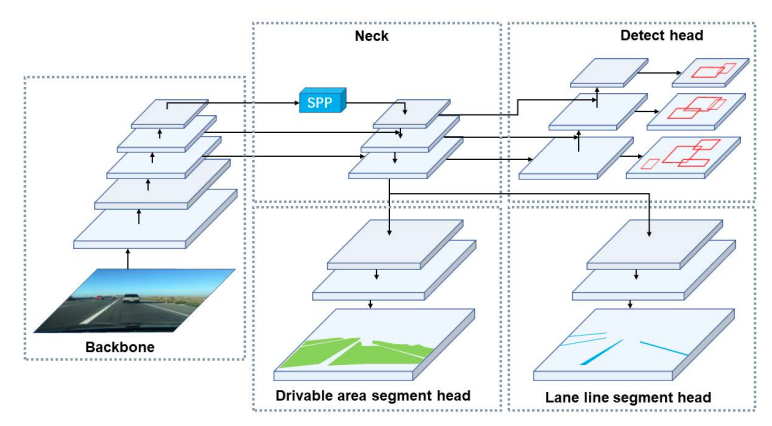
\includegraphics[scale=0.4]{figs/Diseño/YOLOP/yolop-architecture.png}
  \end{center}
  \caption{Arquitectura de YOLOP}
  \label{fig:Arq_YOLOP}
  \vspace{-1.5em}
\end{figure}

YOLOP está compuesto por un codificador para la extracción de características y tres decodificadores para manejar las tareas específicas. Este modelo ha demostrado un rendimiento 
bueno en el desafiante conjunto de datos BDD100K\cite{BDD100K}, logrando el estado del arte en las tres tareas en términos de precisión y velocidad. 

Nosotros utilizaremos los decodificadores de segmentación del área transitable 
y detección de carriles. El decodificador de segmentación del área transitable utiliza los mapas de características
extraídos por el codificador para realizar una predicción semántica a nivel de píxeles. Esto significa que 
para cada píxel de la imagen, el decodificador de segmentación del área transitable predice si el píxel 
pertenece a un área transitable o no. 

Ambos decodificadores, deben de recibir una entrada (W/8,H/8,256):  
\begin{enumerate}
  \item \textbf{W/8 y H/8}: Representa la anchura y la altura de la imagen de entrada, respectivamente, divididas por 8.
  \item \textbf{256}: es el número de 
  canales en el tensor de entrada. En el contexto de las redes neuronales convolucionales, 
  un canal puede ser una característica aprendida (como bordes, texturas, colores, etc.) o una capa de color en una imagen (como rojo, verde, azul en imágenes RGB)
\end{enumerate}

Devuelven una salida de tipo (W,H,2), siendo W la anchura y H la altura de la imagen, solo hay dos canales en cada mapa de características, ya que cada píxel 
representa si pertenece a una clase de objeto o al fondo. 

\subsubsection{Modelo de YOLOP}
\label{sec:Modelo_YOLOP}

YOLOP utiliza una arquitectura de red neuronal CNN. Es un tipo de red neuronal artificial diseñada para procesar datos con una
estructura de cuadrícula, como una imagen. Esta red presenta los diferentes modelos:

\begin{enumerate}
  \item \textbf{End-to-end.pth}: Este archivo se ha construido a partir de la biblioteca Pytorch. 
  \item \textbf{Yolop-320-320.onnx, Yolop-640-640.onnx y Yolop-1020-1020.onnx}: Estos tres archivos se han construido usandO ONNX Runtime.
\end{enumerate}

Dependiendo de que modelo se quiera utilizar, se obtiene resultados diferentes en el ámbito de cómputo y rapidez a la hora de 
realizar la inferencia del modelo. En el código \ref{cod:ejemploYOLOP} se puede encontrar un ejemplo del uso de la red en la página Pytorch dedicada a la red neuronal YOLOP\footnote{\url{https://pytorch.org/hub/hustvl_yolop/}}
y en la figura \ref{f:resultadosYOLOP} se muestra un ejemplo del uso de YOLOP utilizado en la página DebuggerCafe\footnote{\url{https://debuggercafe.com/yolop-for-object-detection-and-segmentation/}}

\begin{code}[h]
  \begin{lstlisting}[language=Python]
    import torch

    # load model
    model = torch.hub.load('hustvl/yolop', 'yolop', pretrained=True)
    
    #inference
    img = torch.randn(1,3,640,640)
    det_out, da_seg_out,ll_seg_out = model(img)
    
  \end{lstlisting}
  \caption[Cargar modelo YOLOP con pesos preentrenados End-to-end.pth]{Ejemplo básico de cómo poder utilizar YOLOP}
  \label{cod:ejemploYOLOP}
  \end{code}  

  \begin{figure}[H]
    \centering
    \begin{minipage}{0.6\textwidth}
      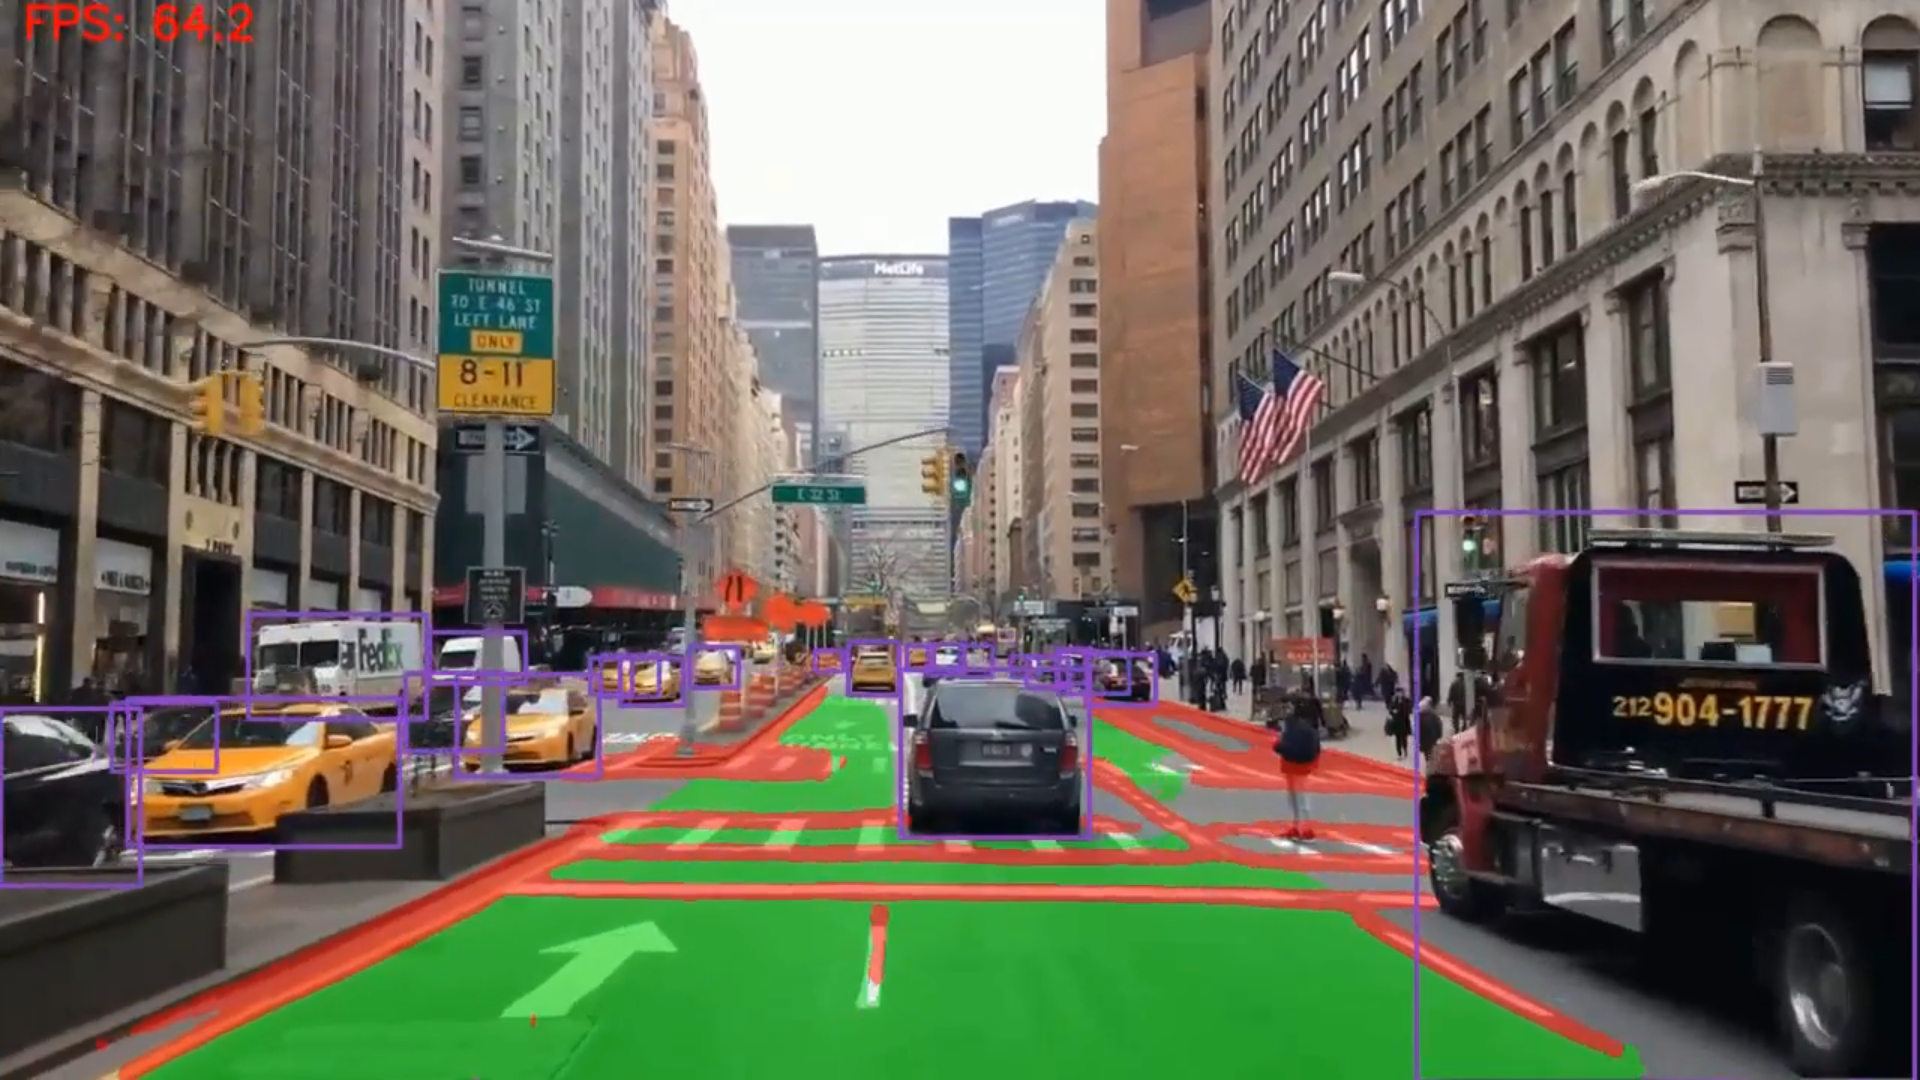
\includegraphics[width=\linewidth]{figs/Plataformas_Desarollo/YOLOP1.png}
    \end{minipage}
    \caption{Resultado de la salida de la red neuronal YOLOP}
    \label{f:resultadosYOLOP}
    \vspace{-1.5em}
  \end{figure}

Por lo que, se utiliza esta red neuronal para poder detectar los carriles que puede tener las áreas transitables en Airsim. 

\section{ROS}
\label{sec:ros}
\textbf{ROS (Robot Operating System)}\footnote{\url{https://www.ros.org/}} es un conjunto de librerías de código abierto utilizadas principalmente para aplicaciones robóticas. 
Podemos definir este middleware como se muestra en la figura \ref{fig:ROS}:

\begin{figure} [H]
    \begin{center}
      
\includegraphics[scale=0.18]{figs/Plataformas_Desarollo/ros-equation.png}
    \end{center}
    \caption{Definición de ROS}
    \label{fig:ROS}
    \vspace{-1.5em}
  \end{figure}


\begin{enumerate}
    \item \textbf{Plumbing}: ROS proporciona una infraestructura de mensajería publicador-subscriptor diseñada para facilitar la construcción sencilla y rápida de sistemas informáticos
    distribuidos.
    \item \textbf{Tools}: ROS proporciona introspección, lanzamiento, depuración, visualización, trazado, registro, reproducción y detener sistemas informáticos distribuidos.
    \item \textbf{Capabilities}: ROS proporciona una amplia colección de bibliotecas que implementan funciones útiles para los robots, por ejemplo, movilidad, manipulación y percepción.
    \item \textbf{Community}: ROS cuenta con el apoyo y la mejora de una gran comunidad, con un fuerte enfoque en la integración y la documentación, gracias a ello, es una ventaja poder
    aprender a cerca de los miles de paquetes que ofrece ROS que están disponibles de desarrolladores de todo el mundo.
\end{enumerate}

Este middleware sigue un modelo parcialmente centralizado de publicación y suscripción, el cual el publicador genera mensajes y eventos asociados a un topic y el subscriptor
es quien se subscribe al topic correspondiente y recibe la información que ha generado el publicador. 

Este tipo sistema es bastante útil ya que permite a los desarrolladores cambiar, añadir o eliminar nodos (programas en ejecución) sin afectar al resto del sistema, facilitando de forma asíncrona
el desarrollo iterativo, permitiendo construir sistemas robóticos complejos, escalables y robustos mejorando la eficiencia y permitiendo el desarrollo y mantenimiento de aplicaciones
robóticas. 

Se utiliza ROS junto con la distribucción Noetic\footnote{\url{https://wiki.ros.org/noetic}} en el desarrollo del TFG para realizar la conexión con el simulador Airsim y el desarrollo del sistema de percepción del seguimiento del carril a través del controlador PID y 
aprendizaje por refuerzo. 


\begin{figure} [H]
    \begin{center}
      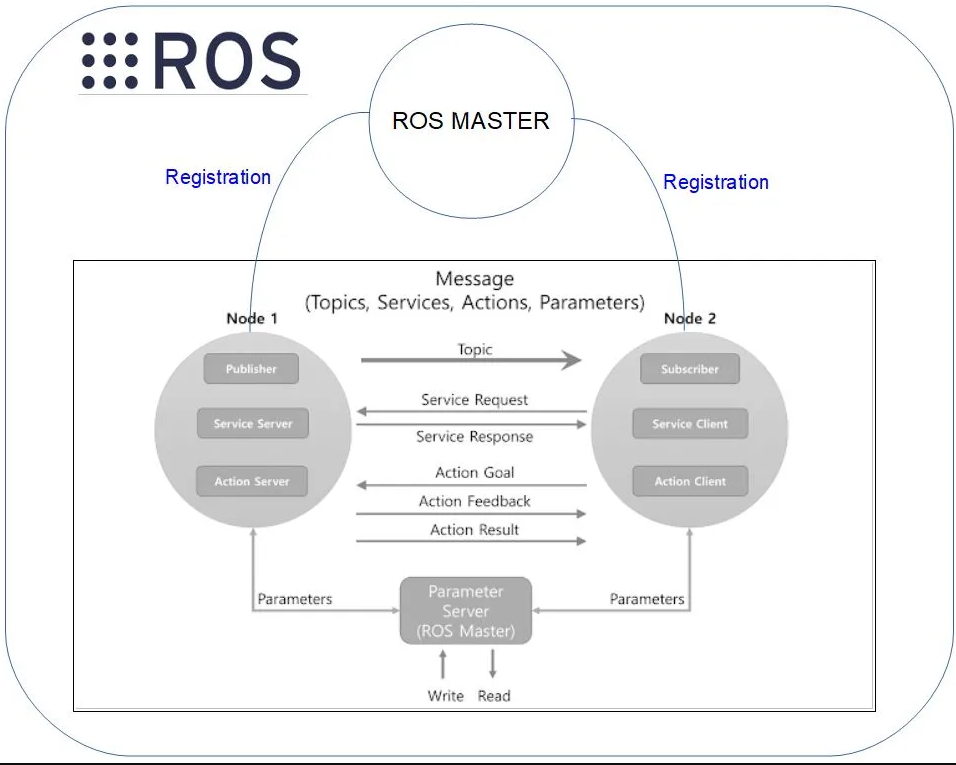
\includegraphics[scale=0.4]{figs/Plataformas_Desarollo/arq_ros.png}
    \end{center}
    \caption{Arquitectura de ROS}
    \label{fig:ArqROS}
  \end{figure}
\subsection{Mavros}
\vspace{-1.5em}
\label{sec:mavros}

\textbf{Mavros}\footnote{\url{http://wiki.ros.org/mavros}} es un paquete formado por \textbf{ROS} y el protocolo de comunicaciones ligero \textbf{MAVLink} (Micro Air Vehicle Link) diseñado por Lorenz Meir\footnote{\url{https://www.technologyreview.es/listas/35-innovadores-con-menos-de-35/2017/inventores/lorenz-meier}} bajo el LGPL licencia. Este protocolo es utilizado para enviar información de estado,
para controlar el vehículo y recibir datos de telemetría. Fácil de implementar en sistemas con recursos limitados, 
lo que lo hace ideal para su uso en drones y otros vehículos aéreos no tripulados.

Ademas, \textbf{Mavros} traduce los mensajes \textbf{ROS} a mensajes \textbf{MAVLink} y viceversa por lo que permite que los datos y comandos fluyan entre \textbf{ROS} y el drone, 
permitiendo un control más sofisticado y una mayor funcionalidad. 

Por lo que, en este TFG se estudia y se analiza sí \textbf{Mavros} se podría utilizar para el control del dron junto con \textbf{PX4 AutoPilot} (\ref{sec:px4}) a través
de Airsim. 

\begin{figure} [H]
  \begin{center}
    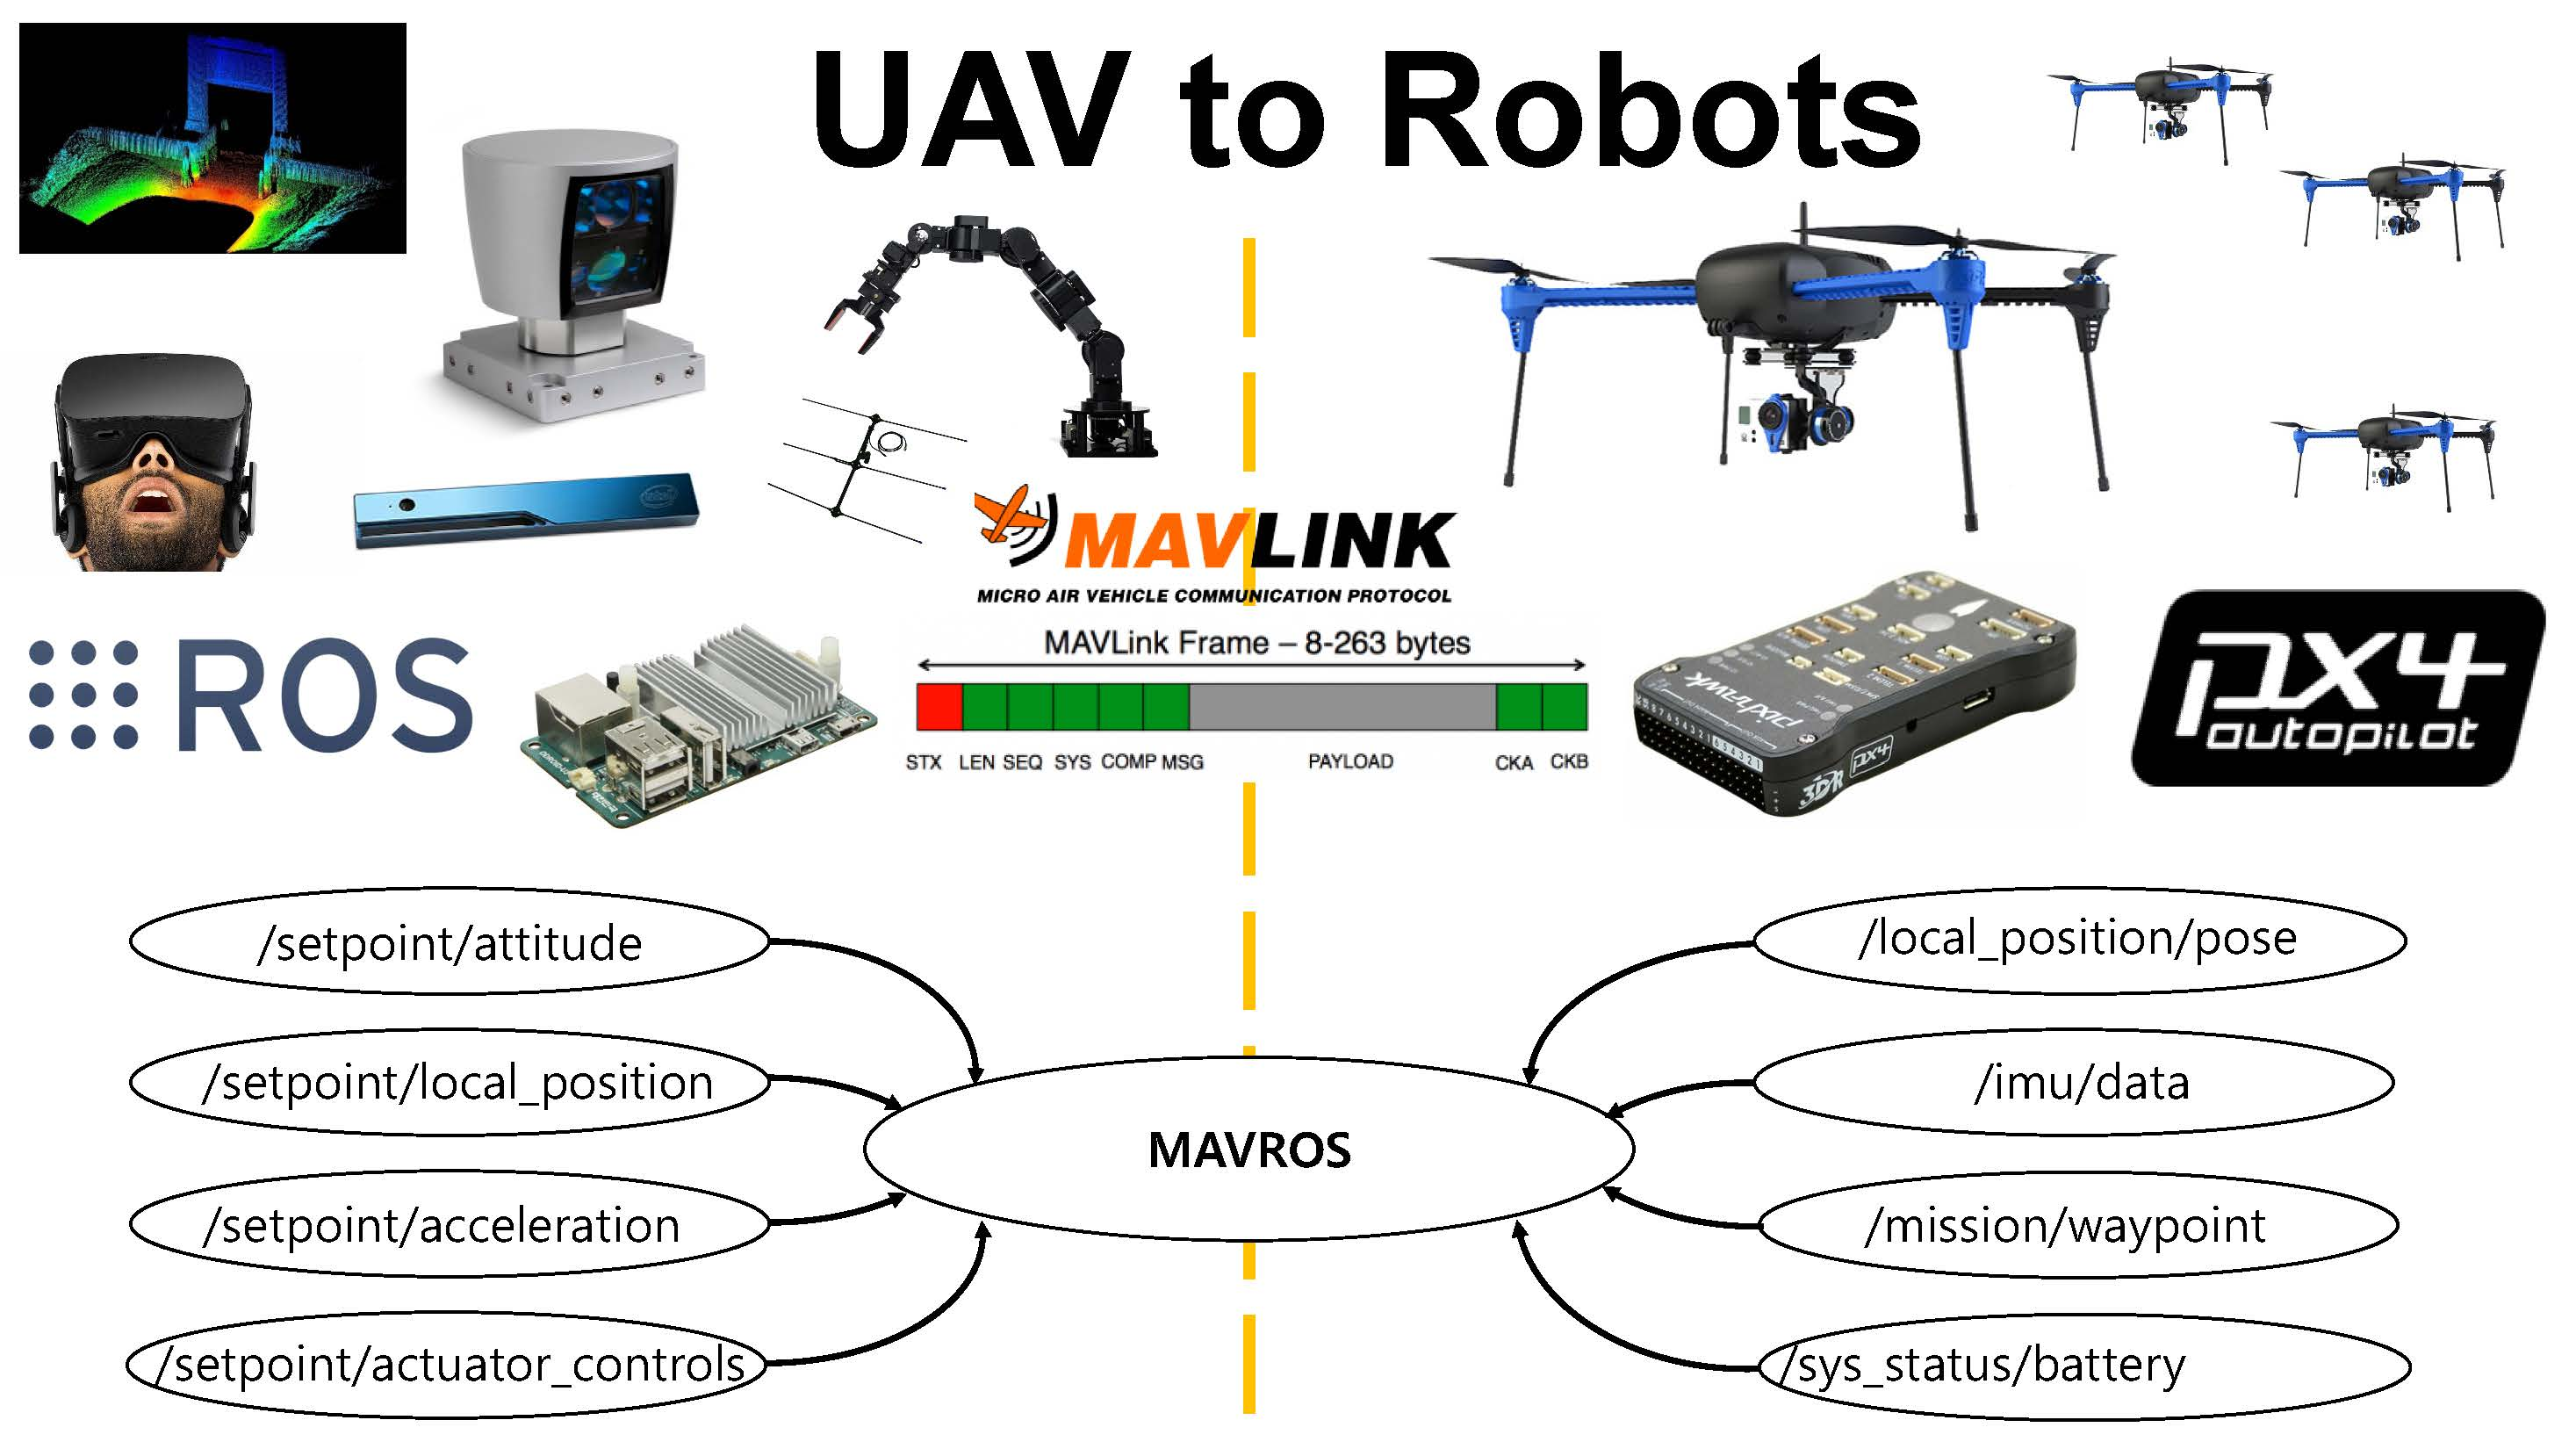
\includegraphics[scale=0.3]{figs/Plataformas_Desarollo/mavros.jpg}
  \end{center}
  \caption{Infraestructura de Mavros}
  \label{fig:InfraROS}
  \vspace{-1.5em}
\end{figure}

\section{Airsim}
\label{sec:Airsim}
El entorno de simulación en el que vamos a estar trabajando será \textbf{Airsim} junto con \textbf{UnRealEngine} de Epic Games\footnote{\url{https://www.unrealengine.com/es-ES}}. \textbf{Airsim}\footnote{\url{https://microsoft.github.io/AirSim/}} es un simulador de código abierto que se utiliza en aplicaciones robóticas 
y aprendizaje automático.
Se construye sobre entornos 3D creados con \textbf{UnRealEngine}, estos entornos son utilizados para simular el mundo real y probar 
cómo los vehículos autónomos se comportarían en diferentes situaciones. \textbf{Airsim} es compatible en varias plataformas como Linux, Windows, macOS y también para Docker y WSL. En nuestro caso,se utilizará en Linux junto
con \textbf{ROS}. 

Por otro lado \textbf{UnRealEngine} es un motor de videojuegos que se utiliza para la creación y simulación de entornos 3D realistas para videojuegos,
películas animadas, experiencias interactivas y de realidad virtual. Es una propuesta innovadora utilizar este tipo de herramientas ya que puedes simular 
comportamientos físicos que se puedan producir en un entorno real. 

Como hemos comentado anteriormente, \textbf{Airsim} es una buena opción de uso si queremos tener comportamientos
similares a un entorno real. Ofrece una variedad de escenarios, tipos de vehículos, sensores y configuraciones del entorno 
según las necesidades u objetivos marcados de cada persona. 
Para ello se debe todo configurar en un fichero de configuración con extensión json denominado settings.json ,lo cual para configurar
el vehículo con nuestras necesidades necesitaremos definir diferentes variables. 

Un archivo settings.json es un archivo de configuración específica de Airsim que define cómo 
se ejecutará la simulación en términos de propiedades del vehículo, configuración de sensores, condiciones climatológicas y más. 

Un archivo settings.json consta de varias secciones: 
\begin{enumerate}
  \item \textbf{SimMode}: Este parámetro define el modo de simulación, se refiere si el modo de simulación es para coches, multirotores o visión de computador.
  \item \textbf{ClockType}: Determina qué tipo de reloj se utiliza para medir el tiempo en la simulación. 
  \item \textbf{Vehicles}:Configuración de  las propiedades de cada vehículo individualmente. Puedes especificar el tipo de vehículo, la posición inicial, la dinámica del vehículo, entre otros.
  \begin{itemize}
    \item \textbf{VehicleType}: En este caso ese parámetro es el tipo de vehículo que utilizaremos en la simulación.
    \item \textbf{UseSerial}: Es para saber si vamos a usar un puerto serial en físico si utilizamos un vehículo en un entorno real.
    \item \textbf{ControlIp}: Esta opción es para especificar si el comportamiento se realizará simulado.
    \item \textbf{ControlPortLocal}: Se especificará el puerto Local. 
    \item \textbf{ControlPortRemote}: Se especificará el puerto Remoto.
    \item \textbf{LocalHostIp}: La dirección IP del ordenador en donde llevaremos la simulación.
    \item \textbf{Sensors}: Permite personalizar la configuración de los sensores simulados, como Lidar, IMU (Unidad de Medición Inercial),GPS y sensor de distancia. 
    \item \textbf{Cameras}: Puedes configurar las cámaras utilizadas en la simulación, especificando sus propiedades como resolución, tipo de lente, posición y orientación relativas al vehículo. 
    
    Se usa una cámara que proporciona una imagen RGB de dimensiones 620x620 píxeles y con
    el flag de PublishToRos a 1 para poder acceder a ella mediante el Airsim ROS Wrapper.
  \end{itemize}
\end{enumerate}

Para más detalles sobre el archivo de settings.json está la paǵina oficial de Airsim\footnote{\url{https://microsoft.github.io/AirSim/settings/}} 

\subsubsection{Escenarios}
\label{sec:airsim}
Los escenarios que ofrece Airsim depende en que sistema operativo nos encontremos, en nuestro caso al utilizar el escenario en Windows 
tenemos más variedad que en comparación con Linux. 

Tiene escenarios desde carreteras y ciudades con coches simulados hasta entornos industriales como almacenes y entornos de montaña con carreteras como se 
muestra en la figura \ref{f:escenarios_airsim}. En este caso
se ha utilizado el escenario Coastline, consiste en un entorno fotorrealista de un recorrido amplio de 2 carriles con ambiente tropical. Con este entorno se obtiene la
información del entorno para realizar el comportamiento sigue carril con el dron. 

Todos estos escenarios se pueden encontrar en las releases de Airsim\footnote{\url{https://github.com/Microsoft/AirSim/releases}} tanto para Windows como para Linux.
En nuestro caso hemos utilizado el escenario Coastline, ya que queremos desarrollar un comportamiento de seguimiento de carril y este escenario ofrece un amplio recorrido de 2 carriles para poder llevarlo
a cabo.

\subsubsection{Sensores}
\label{sec:airsim}
Ofrece sensores como cámaras, barómetros, Imus, GPS, Magnetómetros, sensores de distancia y Lidar.
En nuestro caso utilizaremos como sensores una cámara para poder realizar la detención del carril 
que queremos seguir, el sensor Lidar para saber a que altura se encuentra el dron respecto al suelo y el sensor
GPS para poder obtener la localización del vehículo. 


\begin{figure}[H]
  \centering
  \begin{minipage}{0.45\textwidth}
      \centering
      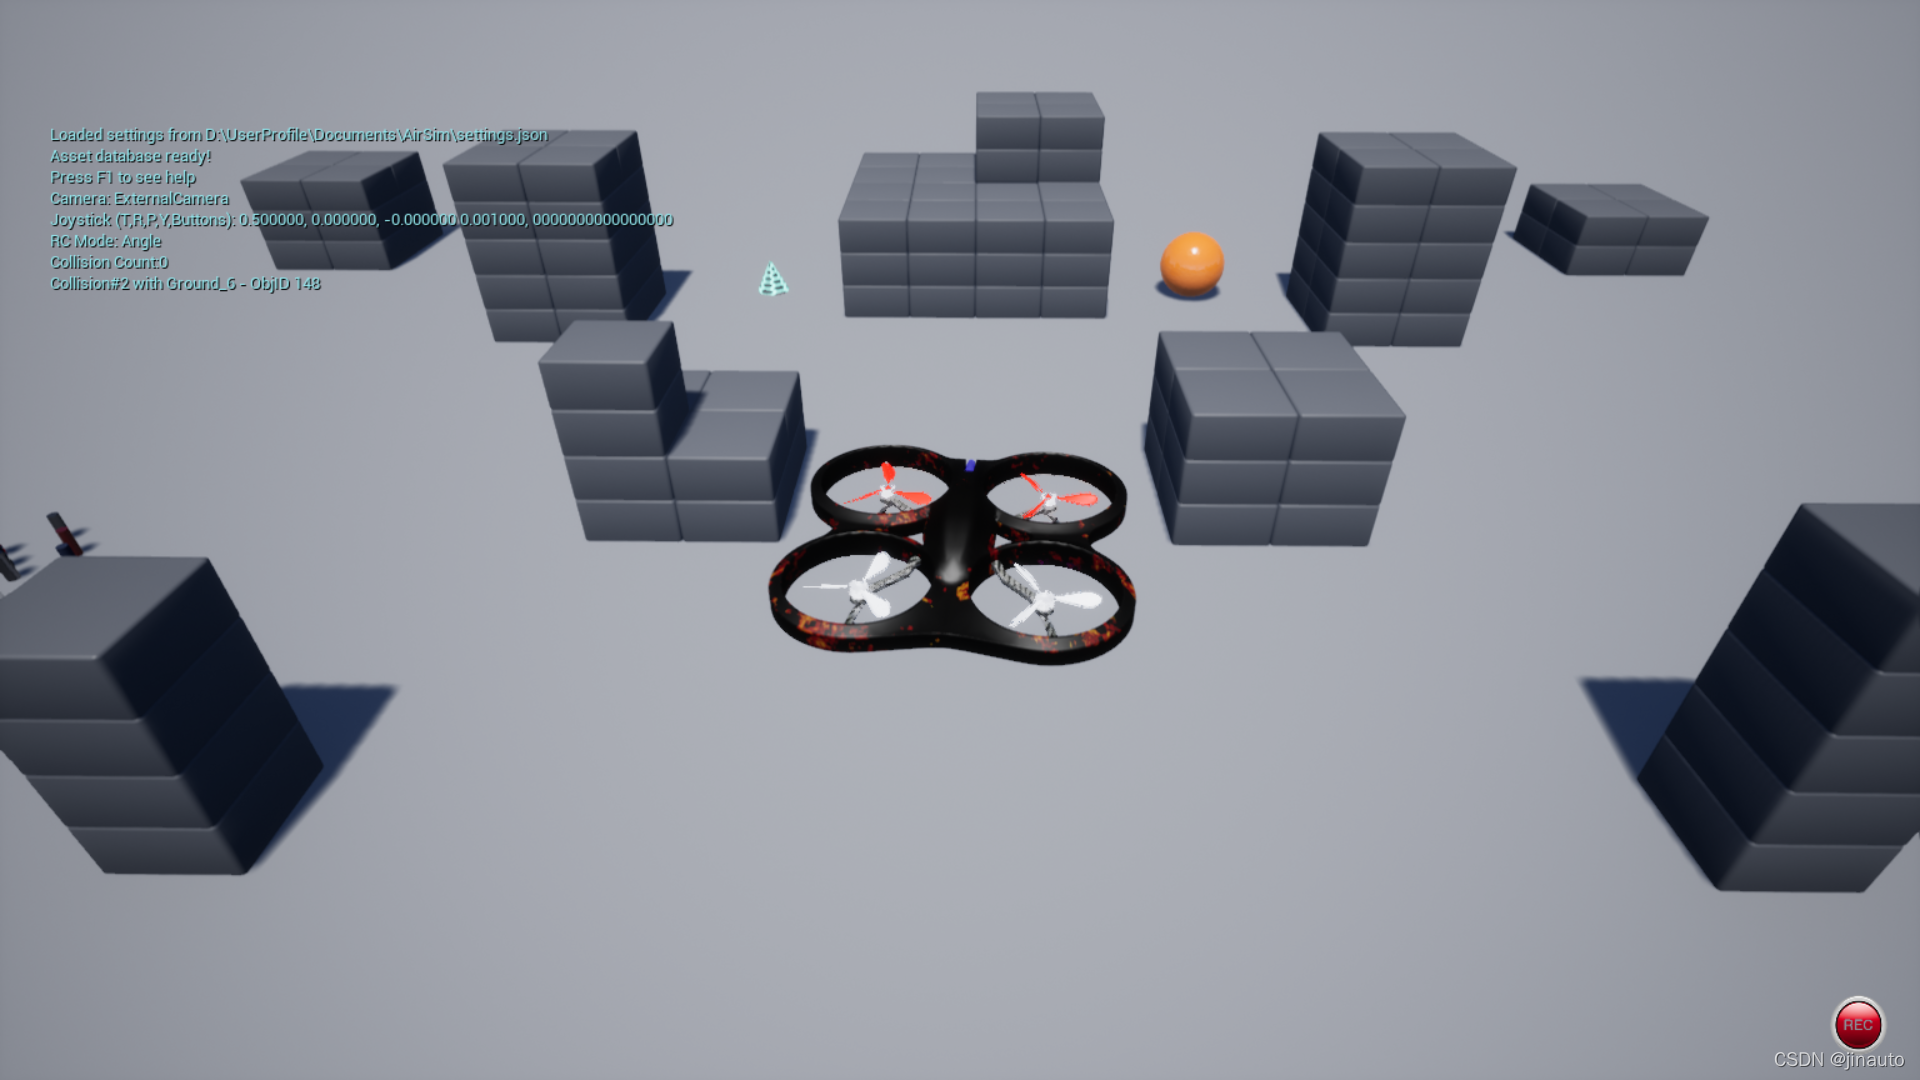
\includegraphics[width=\linewidth]{figs/Plataformas_Desarollo/mapas_airsim/blocks.png}
      \caption*{a) Blocks}
  \end{minipage}%
  \begin{minipage}{0.45\textwidth}
      \centering
      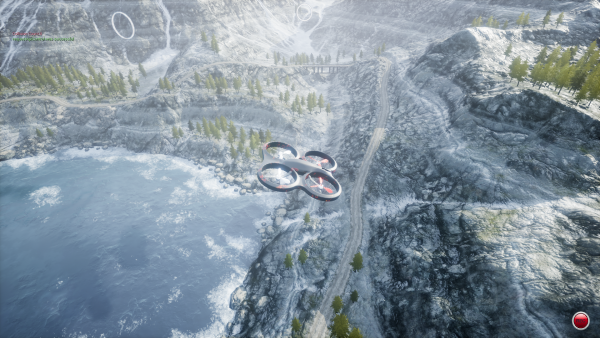
\includegraphics[width=\linewidth]{figs/Plataformas_Desarollo/mapas_airsim/landscapemountains.png}
      \caption*{b) LandscapeMountains}
  \end{minipage}

  \begin{minipage}{0.45\textwidth}
      \centering
      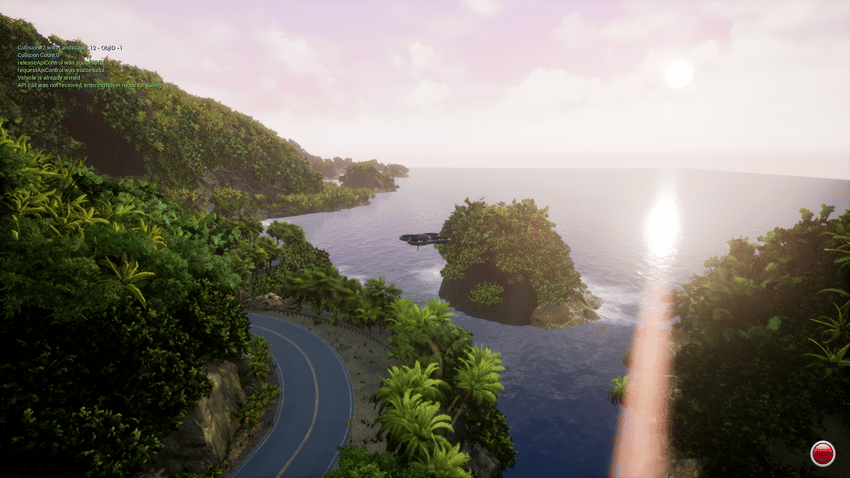
\includegraphics[width=\linewidth]{figs/Plataformas_Desarollo/mapas_airsim/Coastline.png}
      \caption*{c) Coastline}
  \end{minipage}%
  \begin{minipage}{0.45\textwidth}
      \centering
      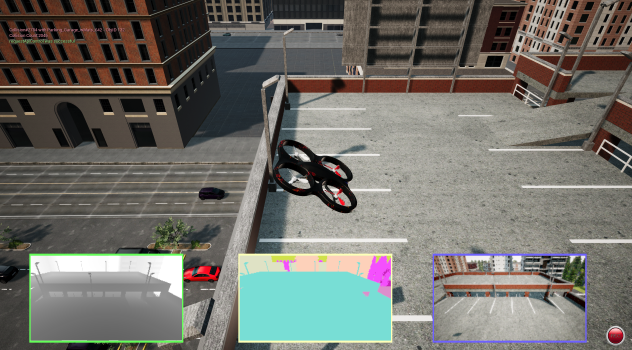
\includegraphics[width=\linewidth]{figs/Plataformas_Desarollo/mapas_airsim/city_airsim.png}
      \caption*{d) City}
  \end{minipage}

  \begin{minipage}{0.45\textwidth}
      \centering
      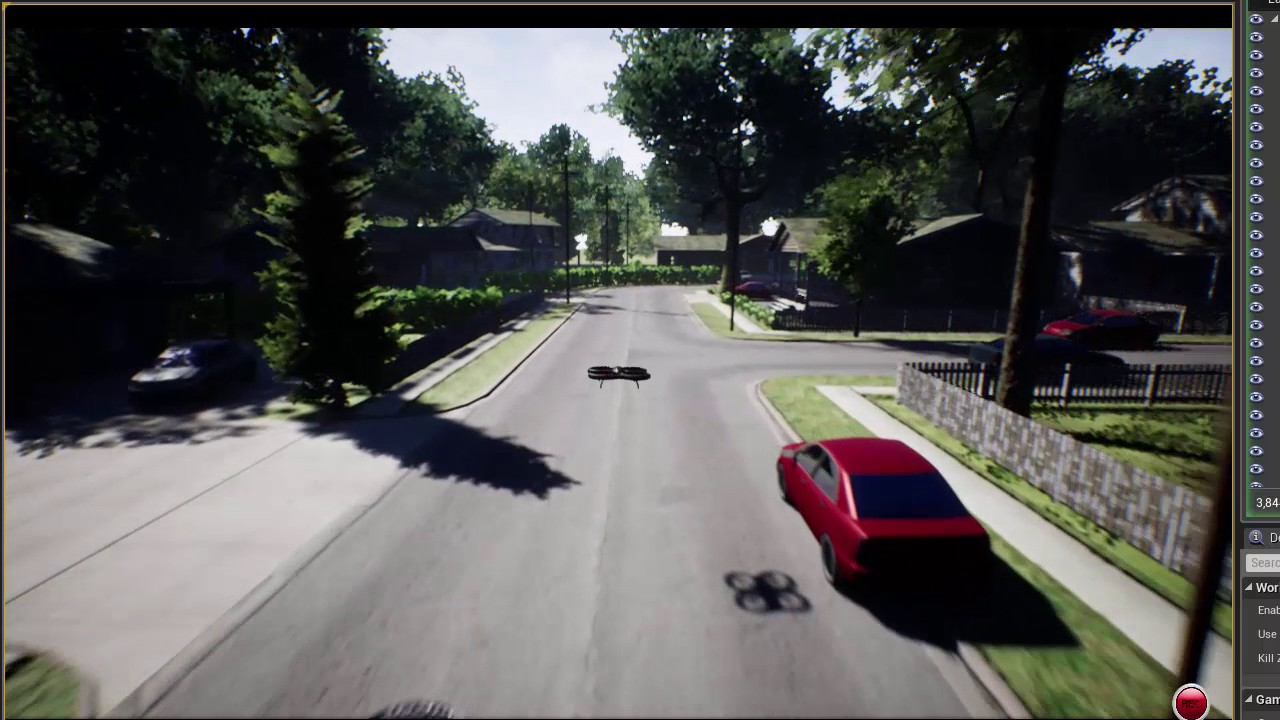
\includegraphics[width=\linewidth]{figs/Plataformas_Desarollo/mapas_airsim/AirsimNH.jpg}
      \caption*{e) Neighborhood}
  \end{minipage}
  \caption{Ejemplos de escenarios en Airsim}
  \label{f:escenarios_airsim}
  \vspace{-1.5em}
\end{figure}


\subsubsection{Tipos de vehículos}
\label{sec:airsim}
\textbf{Airsim} ofrece dos tipos principales de vehículos para la simulación: coches y drones. Dentro de estos tipos se encuentran los subtipos de coches y drones que se puede utilizar.
\begin{enumerate}
  \item \textbf{Coche}
    \begin{itemize}
      \item \textbf{PhysXCar}: Representa un vehículo en tierra con física realista basado en el motor de física PhysX.
      \item \textbf{ArduRover}: Se utiliza para vehículos terrestres que sigan el estándar ArduRover. ArduRover\footnote{\url{https://ardupilot.org/rover/}} 
      se trata de un piloto automático de código abierto utilizado específicamente para vehículos terrestres.
    \end{itemize}
  \item \textbf{Dron}
    \begin{itemize}
      \item \textbf{SimpleFlight}: Representa un dron con un modelo de vuelo simplificado. Este tipo de opción puede ser útil si queremos simular comportamientos 
      de movimiento básico para los drones.
      \item \textbf{PX4Multirotor}: Representa un dron mediante PX4 ArduPilot. 
      \item \textbf{ArduCopter}: Representa un dron pero siguiendo el estándar ArduCopter. ArduCopter\footnote{\url{https://ardupilot.org/copter/}} 
      se trata de un piloto automático de código abierto utilizado para los drones 
    \end{itemize}
  
\end{enumerate}

Como hemos numerado anteriormente, este entorno de simulación tiene un catálogo de vehículos, sensores y
cambios climatológicos dentro del entorno. Nosotros utilizaremos un dron de tipo "SimpleFligh". 

\subsection{Airsim ROS Wrapper}
\label{sec:wrapper}
Utilizaremos el paquete \textbf{Airsim ROS Wrapper}\footnote{\url{https://microsoft.github.io/AirSim/airsim_ros_pkgs/}} para poder acceder a ciertos sensores 
que serán necesarios como es la cámara,el Lidar y el GPS, pero antes de comentar lo que ofrece hablaremos sobre que es un ROS Wrapper. 

\textbf{ROS Wrapper} es un componente que facilita la integración entre dos sistemas o entornos diferentes. Si lo llevamos al contexto de \textbf{ROS}, un wrapper es un nodo o paquete 
que permite que los componentes de \textbf{ROS} se comuniquen con otros sistemas o bibliotecas que no fueron originalmente diseñadas para trabajar con \textbf{ROS}. Este paquete 
puede proporcionar publicación de datos desde el sistema externo a \textbf{ROS} a través de topics, suscripción a topics de \textbf{ROS} para recibir comando o datos, adaptación 
de interfaces de llamada (por ejemplo, entre C++ y Python). 

Por lo tanto, \textbf{Airsim ROS Wrapper} es un paquete de \textbf{ROS} que comunicará \textbf{ROS} y \textbf{Airsim}. Este paquete contiene dos nodos principales 
que han sido realizados mediante la comunidad de Airsim\footnote{\url{https://github.com/microsoft/AirSim}}:
\begin{enumerate}
  \item \textbf{AirSim ROS Wrapper Node}: Este nodo proporciona una interfaz \textbf{ROS} para acceder a los datos del vehículo simulado, por ejemplo, sus sensores, proporcionar velocidades, acceder a su sistema de referencia,etc. 
  \item \textbf{Simple PID Position Controller Node}: Este nodo es un controlador de posición simple basado en un controlador PID (proporcional-derivativo-integral). Ayuda controlar la posición del vehículo 
  simulado en el entorno \textbf{Airsim}.
\end{enumerate}

\subsection{Client Airsim}
\label{sec:Client Airsim}

Airsim ofrece una API implementada para Python demoninada Client Airsim\footnote{\url{https://microsoft.github.io/AirSim/apis/}}, en donde podemos conectarnos con el simulador y tener el control de los sensores y actuadores del vehículo. 
Esta interfaz es bastante útil ya que podemos tener el control del vehículo simulado sin necesidad de tener que utilizar los topics de ROS, es decir, existen métodos los cuales
podemos comandar velocidades al vehículo, tener acceso a los sensores como las cámaras o cambiar configuraciones de la simulación como por ejemplo el clima, el viento, el tiempo del día
o la densidad de tráfico en escenarios donde aparecen coches simulados. 

Esta API se utiliza para el control del dron para realizar su navegación con los controladores PID y en 
el desarrollo de aprendizaje por refuerzo. 

\section{PX4 AutoPilot}
\label{sec:px4}

\textbf{PX4}\footnote{\url{https://docs.px4.io/main/en/}} es una plataforma de software de código abierto para desarrolladores de drones que les permite crear 
y controlar diversos tipos de drones,desde aplicaciones de consumo hasta aplicaciones industriales.
Unas de las principales características que ofrece esta plataforma es el soporte de múltiples tipos de vehículos, como aviones de 
ala fija, multirrotores, helicópteros, rovers y vehículos submarinos, también proporciona diferentes modos de vuelo, 
navegación por puntos de referencias predefinidos, estabilización del vehículo. 

En este trabajo se realiza un análisis respecto a la navegación del dron mediante \textbf{PX4} con el modo de simulación Software in The Loop(SITL) para tener el control del dron junto con 
\textbf{Mavros} y \textbf{Airsim}.
\subsection{Software in The Loop(SITL)}
\label{sec:px4 sitl} 
Este modo de simulación permite a los desarrolladores probar y depurar códigos de control de drones sin necesidad de hardware físico, en lugar de ejecutar el código en un 
vehículo real, este modo simula el comportamiento del vehículo en una computadora. Es especialmente útil durante el desarrollo y la validación de control, navegación y 
planificación de misiones.
Se puede tener diversos entornos de simulación con este modo como Gazebo, Airsim y jMAVSim. Dichos entornos de simulación permiten realizar simulaciones muy realistas y avanzadas 
de cualquier tipo de vehículo simulando una gran variedad de parámetros.

Para poder utilizar PX4 SITL, se debe configurar el entorno de desarrollo adecuado y seguir las instrucciones proporcionadas por la comunidad\footnote{\url{https://docs.px4.io/v1.14/en/simulation/}} .

\subsection{Modos de vuelo}
\label{sec:flight modes} 

PX4 ofrece varios modos de vuelo por ejemplo como Takeoff,Land,Hold, Position, Offboard, etc. Un modo de vuelo define como el usuario puede controlar el vehículo a través de comandos
  y ver que respuesta tiene. 


  \begin{enumerate}
    \item \textbf{TAKEOFF}: Este modo de vuelo permite despegar el dron con una altitud y una velocidad de ascendiente escogida por el usuario con los parametros de PX4 MIS\_TAKEOFF\_ALT y
    MPC\_TKO\_SPEED, dichos parámetros tienen valores por defectos definidos por la plataforma (2.5 m y 1.5 m/s respectivamente). Antes de realizar el despegue el dron será armado 
    para poder realizarlo.

    Una vez se realice el despegue del dron se pasa al modo HOLD 
    \item \textbf{LAND}: Permite aterrizar el dron en donde se encuentre en ese instante, una vez que el dron sea aterrizado, se desarmará por defecto. En este modo se puede cambiar por ejemplo
    la tasa de descenso durante se realiza el aterrizaje del dron con el parametro MPC\_LAND\_SPEED, tiempo en segundos para que se realice el desamardo del dron si se establece dicho tiempo
    con un valor de -1 el dron no se desarmará cuando aterrice.
    
    Cuando de realice este modo de vuelo por defecto se cambiará al modo de POSITION

    \item \textbf{HOLD}: A partir de este modo de vuelo podemos parar el dron manteniendolo en el aire con su actual posición GPS y altitud. Este modo puede ser bastante útil para cuando se quiere
    pausar una mision o reiniciar el comportamiento que se quiera realizar. 

    \item \textbf{POSITION}: Es un modo de vuelo manual el cual puedes controlar el DRON mediante un joystick, dicho vuelo controla la posición del dron cuando comandemos velocidades 
    mediante el joystick.

    \begin{figure} [H]
      \begin{center}
        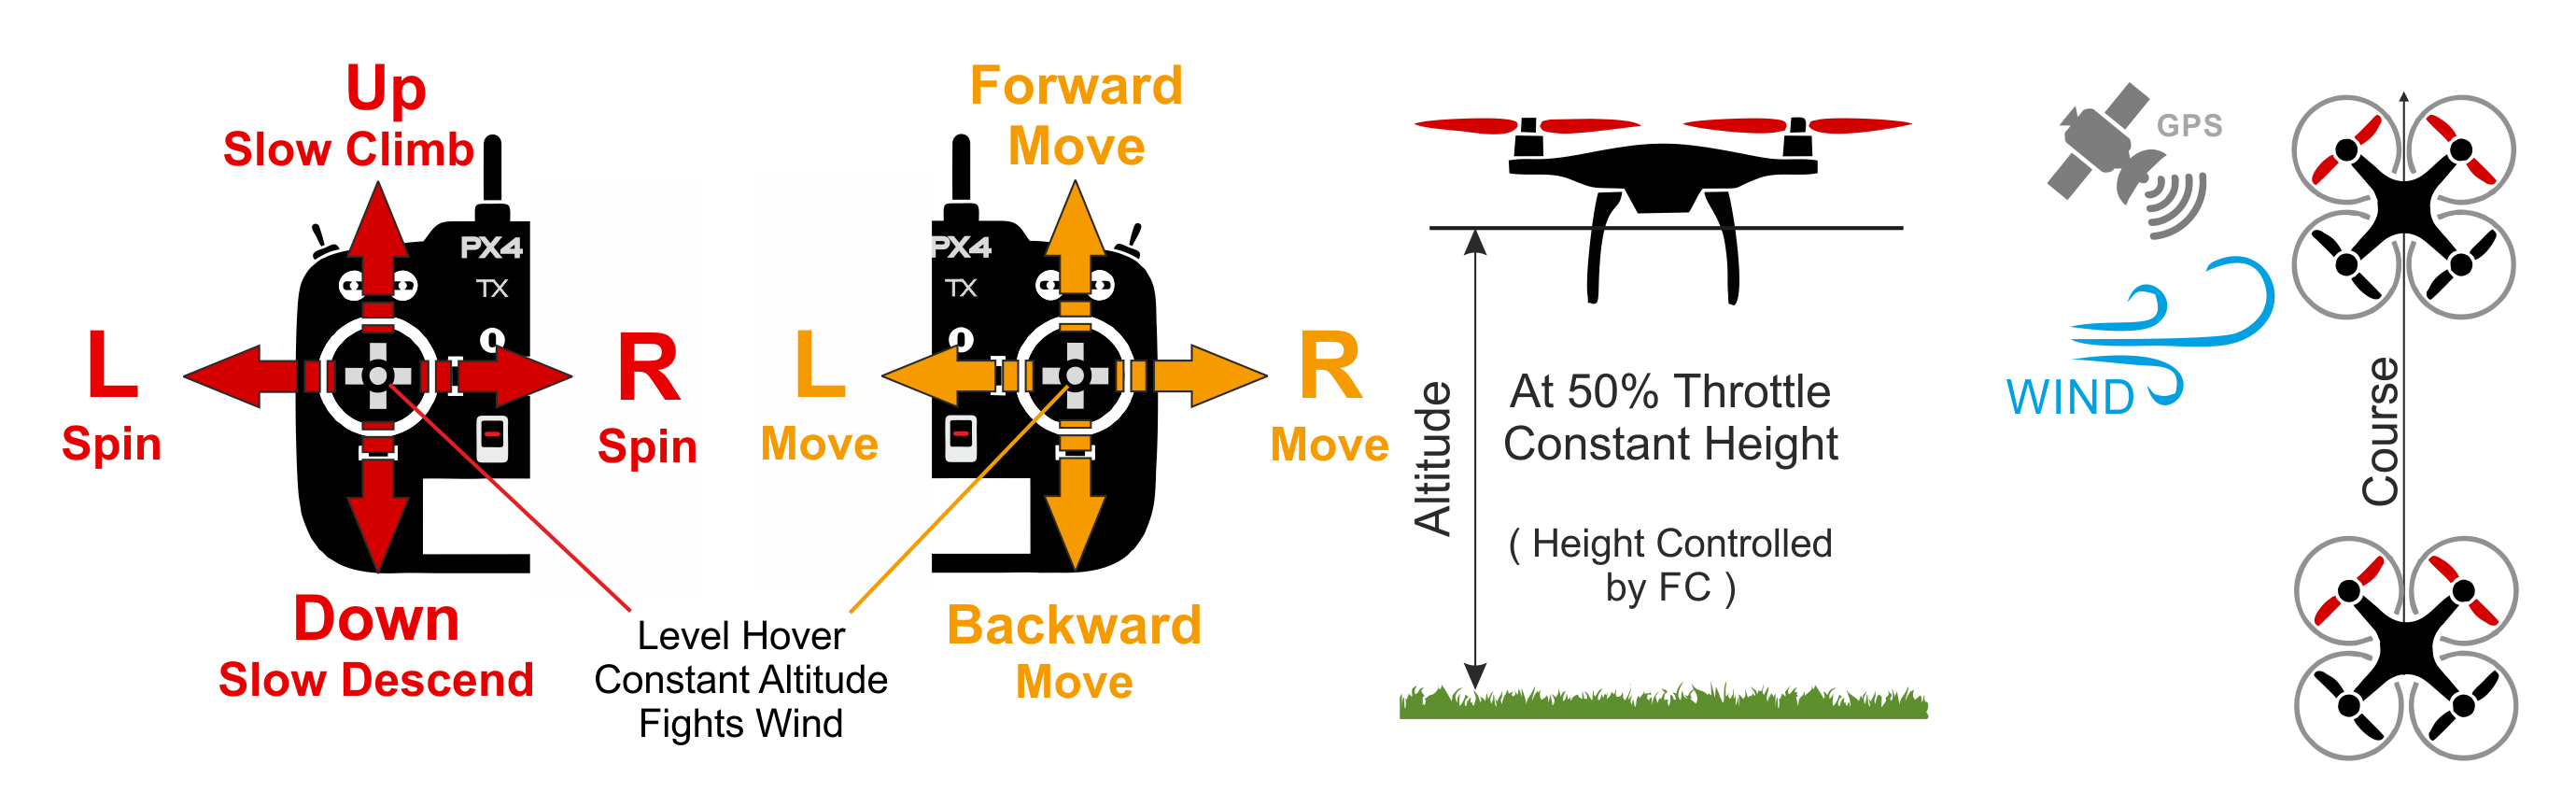
\includegraphics[scale=0.6]{figs/Diseño/PX4/position_MC.png}
      \end{center}
      \caption{Diagrama del comportamiento del modo de vuelo Position}
      \label{fig:position_mode_px4}
      \vspace{-1.5em}
    \end{figure}

    \item \textbf{OFFBOARD}: Con este modo de vuelo se puede controlar el movimiento y la altitud del vehículo a partir de comandos de posición, velocidad, aceleración, altitud, velocidades de 
    altitud o puntos de ajuste de empuje/torque. 

    Dichos comandos debe ser una secuencia de mensajes de setpoint MavLink o a través de topics mediante ROS con Mavros.

    En este modo, PX4 debe recibir una secuencia de mensajes continua. Si en algún momento dejamos de publicar mensajes, el control externo de PX4 dejará de estar en el modo OFFBOARD después
    de pasar un tiempo de espera establecido por el parámetro COM\_OF\_LOOS\_T (por defecto esta establecido a 1 s) e intentará aterrizar o realizar alguna acción de seguridad (dichas acciones 
    de seguridad vienen definidas en la seccion de Failsafes en PX4 Autopilot\footnote{\url{https://docs.px4.io/v1.14/en/config/safety.html}}). La acción dependerá
    si el control RC está disponible, si este control esta disponible pasará a otro tipo de modo de vuelo definido en el parámetro COM\_OBL\_RC\_ACT. 

    Para comandar las velocidades al vehículo mediante Mavros, se tendrá que utilizar el topic denominado \texttt{/mavros/setpoint\_velocity/cmd\_vel\_unstamped} dicho topic utiliza un marco de coordenadas
    por defecto definido en el archivo de configuración de px4.config.yaml LOCAL\_NED. Si se quiere que el marco de coordenadas se mueva con el 
    cuerpo del dron, se tiene que utilizar el marco de coordenadas BODY\_NED
  
    Los marcos de coordenadas que ofrece Mavros se puede ver a través del servicio SetMavFrame.srv\footnote{\url{https://github.com/mavlink/mavros/blob/master/mavros_msgs/srv/SetMavFrame.srv}}
  \end{enumerate}
  
\section{QGroundControl}
\label{sec:QGroundControl} 

\textbf{QGroundControl}\footnote{\url{http://qgroundcontrol.com}} es una plataforma de software que proporciona un control completo de vuelo 
y configuraciones de vehículos para drones por \textbf{PX4 ArduPilot}. Además, ofrece un control total durante el vuelo y permite la planificación de vuelos autónomos 
mediante la definición de puntos de referencia, se muestra la posición del vehículo junto con su trayectoria, los puntos de referencia y los instrumentos del vehículo. 
Es una opción cómoda para poder visualizar tu vehículo y querer cambiar parámetros del vehículo mediante esta aplicación y poder teleoperar el vehículo a través de un mando joystick.
Funciona en diferentes plataformas como Windows, macOS, Linux,iOS y dispositivos Android, en nuestro caso lo utilizaremos en Linux. 

\begin{figure} [H]
  \begin{center}
    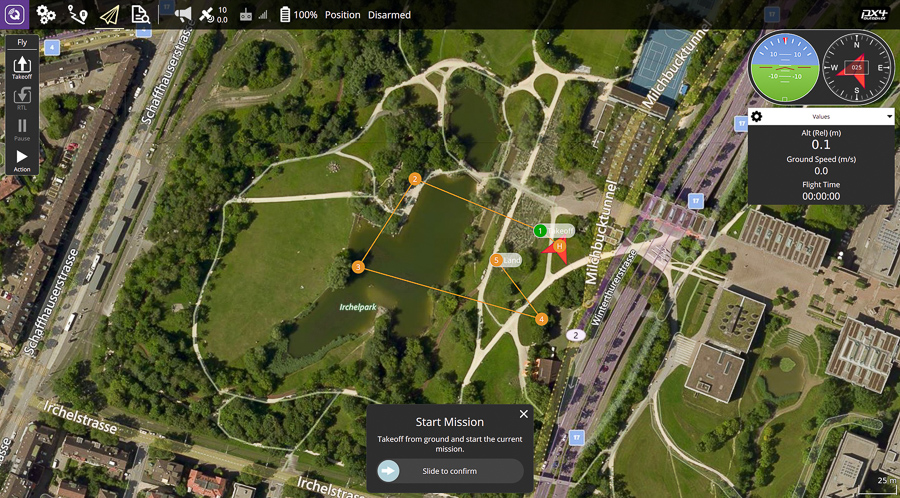
\includegraphics[scale=1.2]{figs/Plataformas_Desarollo/software-qgc.jpg}
  \end{center}
  \caption{QGroundControl}
  \label{fig:QGroundControl}
  \vspace{-1.5em}
\end{figure}


































